\documentclass[12pt]{article}%
\usepackage{amsfonts}
\usepackage{fancyhdr}
\usepackage{comment}
\usepackage[a4paper, top=2.5cm, bottom=2.5cm, left=2.2cm, right=2.2cm]%
{geometry}
\usepackage{times}
\usepackage{amsmath}
\usepackage{changepage}
\usepackage{amssymb}
\usepackage{graphicx}
\usepackage{listings}
\usepackage{color}
\usepackage{hyperref}%
\setcounter{MaxMatrixCols}{30}
\newtheorem{theorem}{Theorem}
\newtheorem{acknowledgement}[theorem]{Acknowledgement}
\newtheorem{algorithm}[theorem]{Algorithm}
\newtheorem{axiom}{Axiom}
\newtheorem{case}[theorem]{Case}
\newtheorem{claim}[theorem]{Claim}
\newtheorem{conclusion}[theorem]{Conclusion}
\newtheorem{condition}[theorem]{Condition}
\newtheorem{conjecture}[theorem]{Conjecture}
\newtheorem{corollary}[theorem]{Corollary}
\newtheorem{criterion}[theorem]{Criterion}
\newtheorem{definition}[theorem]{Definition}
\newtheorem{example}[theorem]{Example}
\newtheorem{exercise}[theorem]{Exercise}
\newtheorem{lemma}[theorem]{Lemma}
\newtheorem{notation}[theorem]{Notation}
\newtheorem{problem}[theorem]{Problem}
\newtheorem{proposition}[theorem]{Proposition}
\newtheorem{remark}[theorem]{Remark}
\newtheorem{solution}[theorem]{Solution}
\newtheorem{summary}[theorem]{Summary}
\newenvironment{proof}[1][Proof]{\textbf{#1.} }{\ \rule{0.5em}{0.5em}}

\newcommand{\Q}{\mathbb{Q}}
\newcommand{\R}{\mathbb{R}}
\newcommand{\C}{\mathbb{C}}
\newcommand{\Z}{\mathbb{Z}}


\lstset{frame=tb,
  language=Bash,
  aboveskip=3mm,
  belowskip=3mm,
  showstringspaces=false,
  columns=flexible,
  basicstyle={\small\ttfamily},
  numbers=none,
  numberstyle=\tiny\color{gray},
  keywordstyle=\color{blue},
  commentstyle=\color{dkgreen},
  stringstyle=\color{mauve},
  breaklines=true,
  breakatwhitespace=true,
  tabsize=3
}

\begin{document}

\title{Single Node Hadoop 3.0.3 setup on Linux Mint 18 (Sarah)}
\author{Aditya Singh Rathore, 2017MSBDA001}
\date{\today}
\maketitle
\section{Prerequisites}
Hadoop is a big data storage and analytics framework that is built on top of the Java TM platform and runs on the Java Virtual Machine. Thus installation of JDK is a must. Also we need to setup passphraseless SSH server in order to access the cluster.

\subsection{Installing JDK 8}
\begin{enumerate}
\item Open terminal and type the following command to add Oracle's PPA,
\begin{lstlisting}
$ sudo add-apt-repository ppa:webupd8team/java
$ sudo apt-get update
\end{lstlisting}
\item Now go on and install JDK 8 on your Machine
\begin{lstlisting}
$ sudo apt-get install oracle-java8-installer
\end{lstlisting}
\item Check if the installation is working type the following command
\begin{lstlisting}
$ javac -version
\end{lstlisting}
You will get your JDK version as output.\\
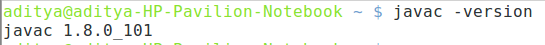
\includegraphics[width=0.8\textwidth]{javac.png}
\end{enumerate}
\subsection{Setting JAVA\_HOME environment Variable and Adding Java to your PATH}
\begin{enumerate}
\item  Open terminal and go to home directory.\\
\lstinline{$ cd ~}
\item  Now open the .bashrc file in your preferred text editor (I am using gedit)\\
\lstinline{$ gedit .bashrc}
\item Add the following lines to the bottom of your .bashrc file.\\
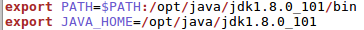
\includegraphics[width=0.8\textwidth]{img1.png}
\item  Compile your .bashrc to make your changes permanent.\\
\lstinline{$ source .bashrc}
\end{enumerate}
\subsection{Setting up passphraseless SSH}
\begin{enumerate}
\item If you have not installed SSH software you will need to install it.\\
\lstinline{$ sudo apt-get install ssh}\\
\lstinline{$ sudo apt-get install pdsh}\\
\item Now in order to  ssh to localhost without a passphrase (Empty password), execute the following commands:\\
\lstinline{$ ssh-keygen -t rsa -P '' -f ~/.ssh/id_rsa}\\
\lstinline{$ cat ~/.ssh/id_rsa.pub >> ~/.ssh/authorized_keys}\\
\lstinline{$ chmod 0600 ~/.ssh/authorized_keys}
\end{enumerate}

\section{Downloading and Installing Hadoop 3.0.3}
\subsection{Downloading Hadoop}
Type the following command to download Hadoop 3.0.3 binary tar file to your machine. It will be downloaded to your home directory.\\
\lstinline{$ wget http://www-eu.apache.org/dist/hadoop/common/hadoop-3.0.3/hadoop-3.0.3.tar.gz}\\
Or to get the latest version go to \url{http://hadoop.apache.org/releases.html}

\subsection{Installing Hadoop}
\begin{enumerate}
\item Unpack the downloaded tar file to /usr/local\\
\lstinline{$ tar -xvf articles.tar -C /usr/local/}
\item A new directory named Hadoop will appear in /usr/local/ directory. If it's Hadoop3.0.3 rename it to Hadoop.\\
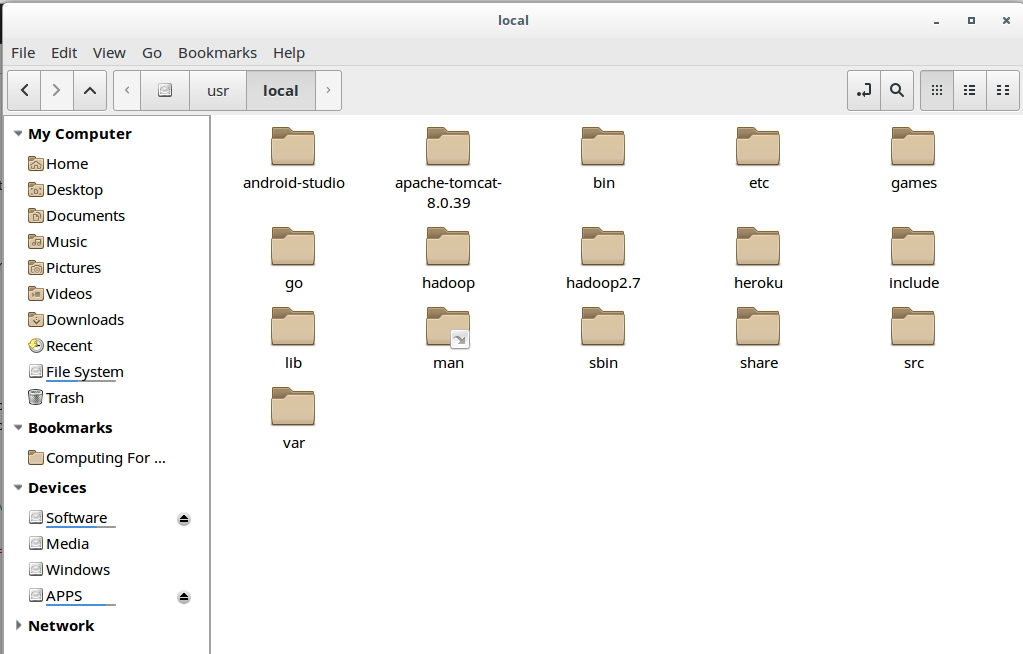
\includegraphics[width=0.8\textwidth]{dir1.png}
\item Now it's time to set the Hadoop specific environment variable. open .bashrc for editing.
\lstinline{$ cd ~}
\lstinline{$ gedit .bashrc}
\item Add the following lines to your .bashrc\\
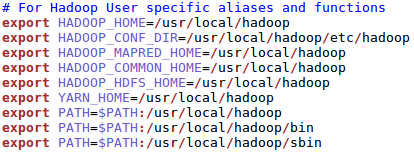
\includegraphics[width=0.8\textwidth]{hadoopenv.png}
\item  Compile your .bashrc to make your changes permanent.\\
\lstinline{$ source .bashrc}
\item  To check if it worked out type the following command.\\
\lstinline{$ hadoop version}
\item  Your output will be something like.\\
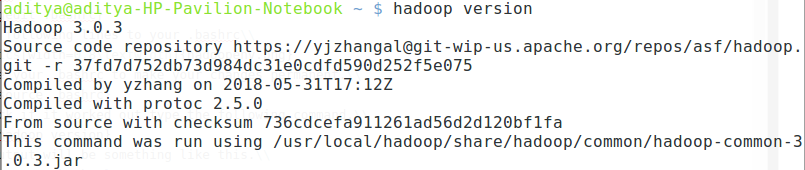
\includegraphics[width=0.8\textwidth]{hadver.png}
\end{enumerate}
\section{HDFS and Yarn Configuration}
We have all the Hadoop binaries on our system but that's not it yet. In order to get Hadoop up and running we have to specify certain properties and configurations. Which is easily done with a little bit of XML hacking.\\\\
Change to hadoop configuration directory\\
\lstinline{$ cd /usr/local/hadoop/etc/hadoop}
\subsection{Edit hadoop-env.sh}
\begin{enumerate}
\item Open hadoop-env.sh for editing.\\
\lstinline{$ gedit hadoop-env.sh}
\item Add the following line to point Hadoop installation towards your JDK (Version may change).\\
\lstinline{export JAVA_HOME=/opt/java/jdk1.8.0_101}
\end{enumerate}

\subsection{Edit core-site.xml}
This file informs Hadoop daemon
where NameNode runs in the cluster.
\begin{enumerate}
\item Open core-site.xml for editing.\\
\lstinline{$ gedit core-site.xml}
\item Add the following properties in between the $<$configuration$>$ and $<$/configuration$>$ tags.\\
\begin{lstlisting}
<configuration>
	<property>
		<name>fs.defaultFS</name>
		<value>hdfs://localhost:9000</value>
	</property>
</configuration>
\end{lstlisting}

\item Complete file will look like below:\\
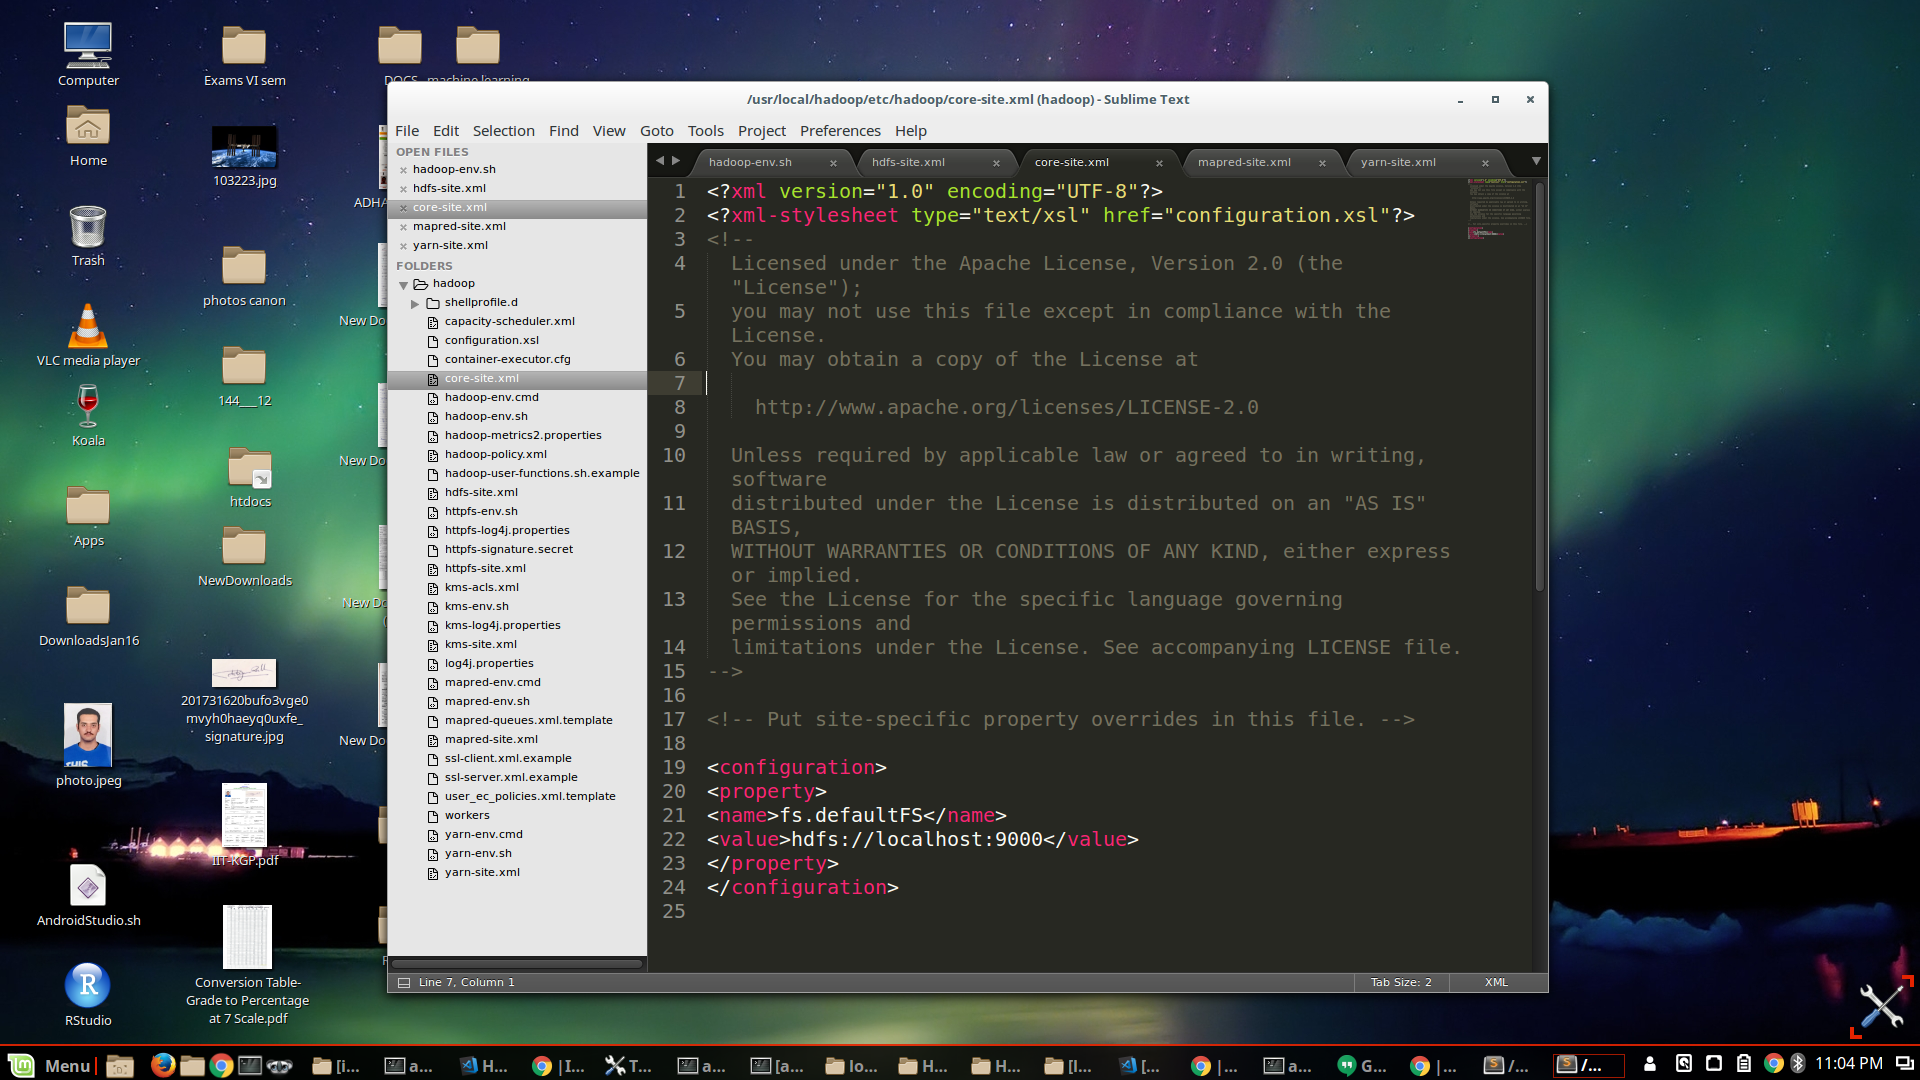
\includegraphics[width=0.8\textwidth]{core-site.png}
\end{enumerate}


\subsection{Edit hdfs-site.xml}
This file contains configuration
settings of various HDFS daemons (i.e. NameNode, DataNode, Secondary
NameNode). It also includes the replication factor and block size of
HDFS.
\begin{enumerate}
\item Open hdfs-site.xml for editing.\\
\lstinline{$ gedit hdfs-site.xml}
\item Add the following properties in between the $<$configuration$>$ and $<$/configuration$>$ tags.\\
\begin{lstlisting}
<configuration>
	<property>
		<name>dfs.replication</name>
		<value>1</value>
	</property>
</configuration> 
\end{lstlisting}
\item Complete file will look like below:\\
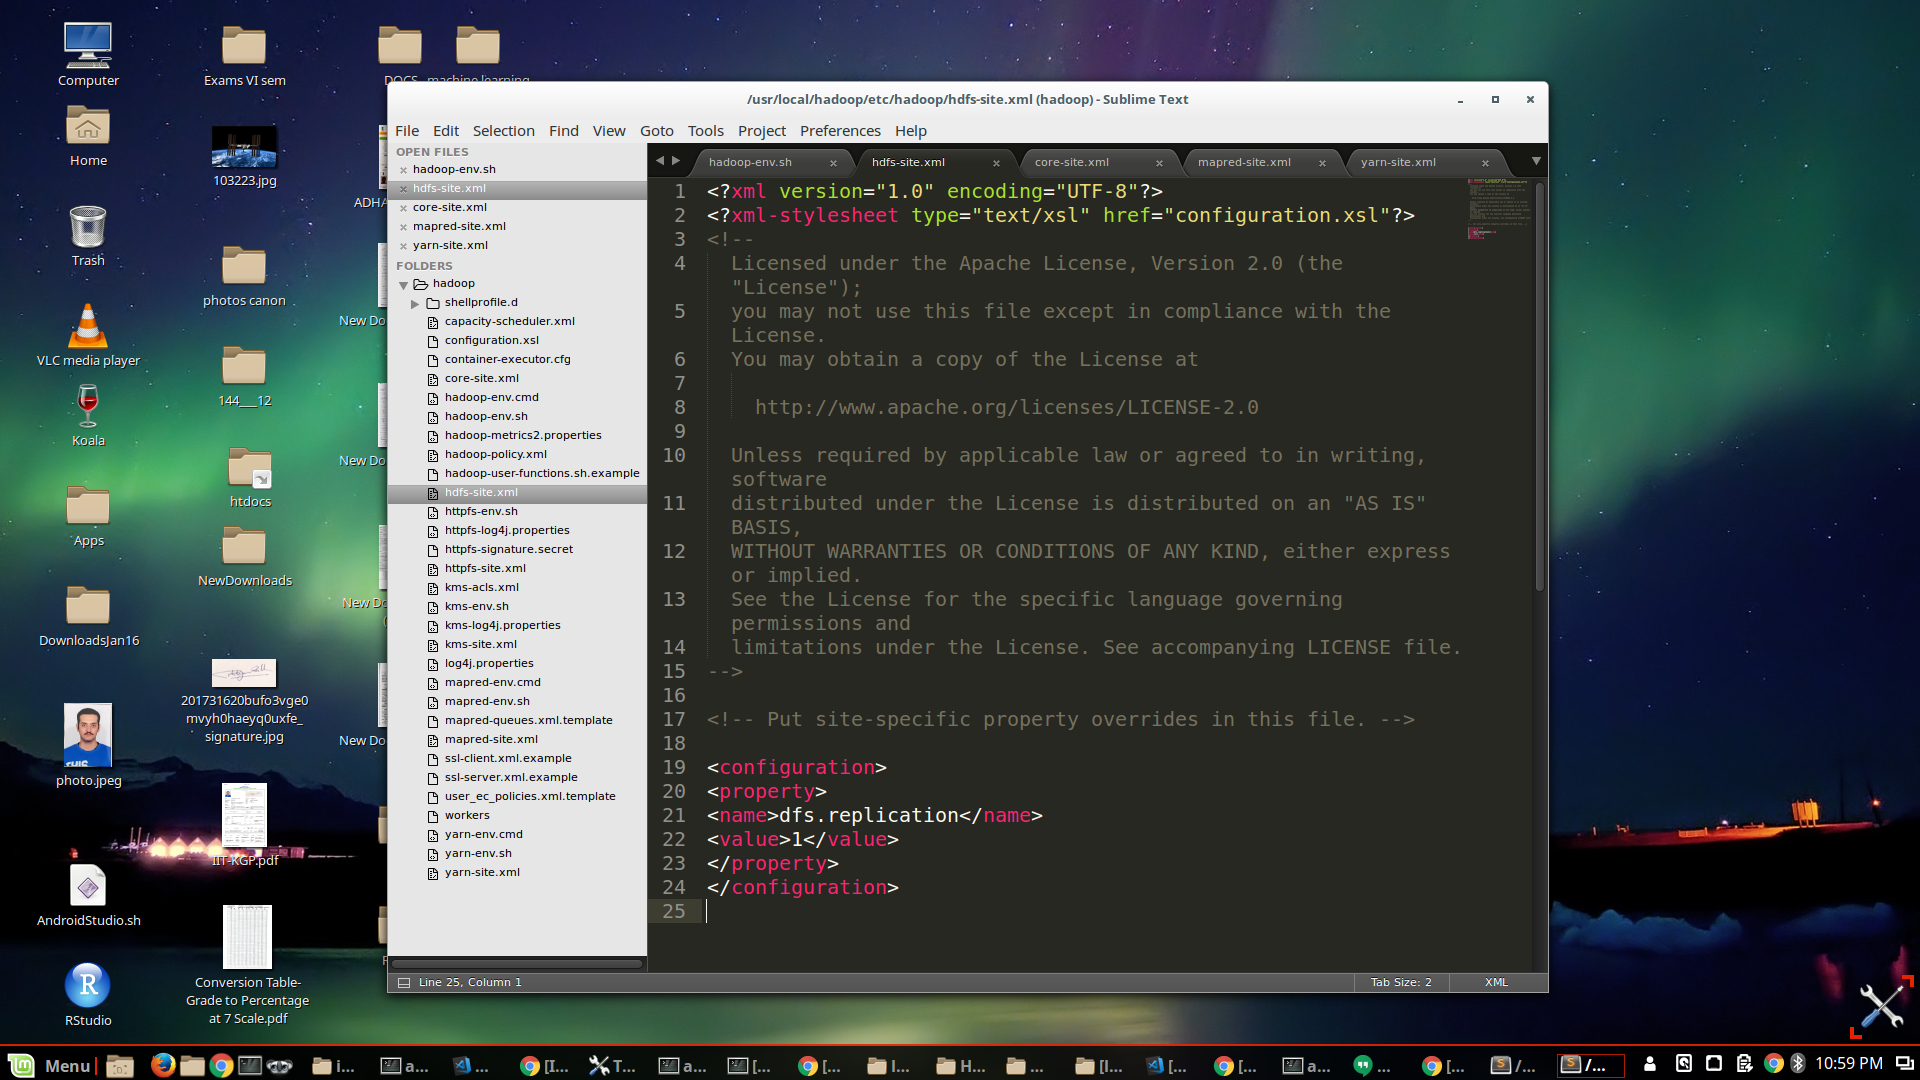
\includegraphics[width=0.8\textwidth]{hdfs-env.png}
\end{enumerate}

\subsection{Edit mapred-site.xml}
This file contains configuration settings of MapReduce application like number of JVM that can run in parallel, the size of the mapper and the reducer
process, CPU cores available for a process, etc.\\
If mapred-site.xml file is not available. So, we have to
create the mapred-site.xml fileusing mapred-site.xml template.
\begin{enumerate}
\item If mapred-site.xml is not avaliable create it from mapred-site.xmltemplate.\\
\lstinline{$ cp mapred-site.xml.template mapred-site.xml}
\item Open mapred-site.xml for editing.\\
\lstinline{$ gedit mapred-site.xml}
\item Add the following properties in between the $<$configuration$>$ and $<$/configuration$>$ tags.\\
\begin{lstlisting}
<configuration>
    <property>
        <name>mapreduce.framework.name</name>
        <value>yarn</value>
    </property>
    <property>
        <name>mapreduce.application.classpath</name>
        <value>$HADOOP_MAPRED_HOME/share/hadoop/mapreduce/*:$HADOOP_MAPRED_HOME/share/hadoop/mapreduce/lib/*</value>
    </property>
</configuration> 
\end{lstlisting}
\item Complete file will look like below:\\
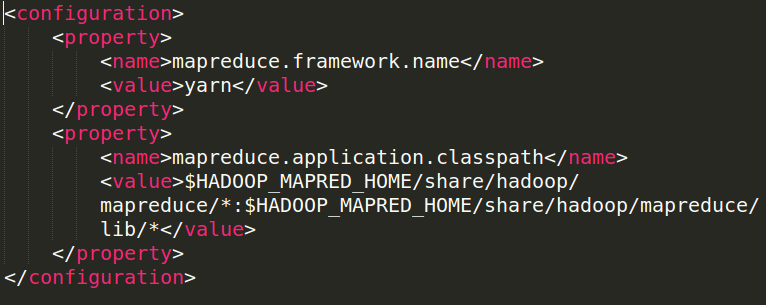
\includegraphics[width=0.8\textwidth]{mapredxml.png}
\end{enumerate}

\subsection{Edit yarn-site.xml}
This file contains configuration
settings of ResourceManager and NodeManager like application
memory management size ,the operation needed on program and
algorithm,
\begin{enumerate}
\item Open yarn-site.xml for editing.\\
\lstinline{$ gedit yarn-site.xml}
\item Add the following properties in between the $<$configuration$>$ and $<$/configuration$>$ tags.\\
\begin{lstlisting}
<configuration>
    <property>
        <name>yarn.nodemanager.aux-services</name>
        <value>mapreduce_shuffle</value>
    </property>
    <property>
        <name>yarn.nodemanager.env-whitelist</name>
        <value>JAVA_HOME,HADOOP_COMMON_HOME,HADOOP_HDFS_HOME,HADOOP_CONF_DIR,CLASSPATH_PREPEND_DISTCACHE,HADOOP_YARN_HOME,HADOOP_MAPRED_HOME</value>
    </property>
</configuration>
\end{lstlisting}
\item Complete file will look like below:\\
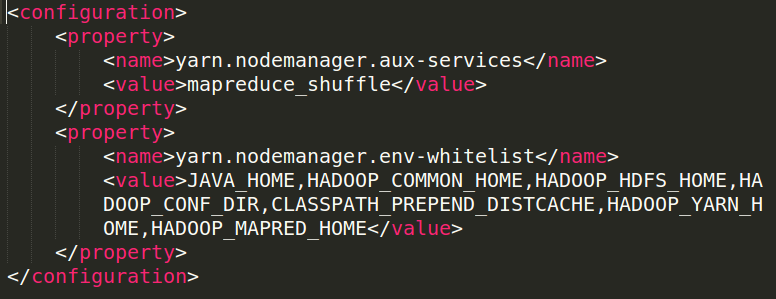
\includegraphics[width=0.8\textwidth]{yarnxml.png}
\end{enumerate}

\section{Running Hadoop Services}
Now since we have added all the the Hadoop binaries and shell script which are present in \emph{/usr/local/hadoop/bin and in /usr/local/hadoop/sbin} to our PATH. We can directly run those binaries and scripts from terminal by just typing in their names.
\begin{enumerate}
\item Firstly we need to SSH to localhost\\
\lstinline{$ ssh localhost}\\
You will see output like below. You are taken to the BASH terminal of your machine but this time commands will run via a SSH connection to localhost (or 127.0.0.1).\\
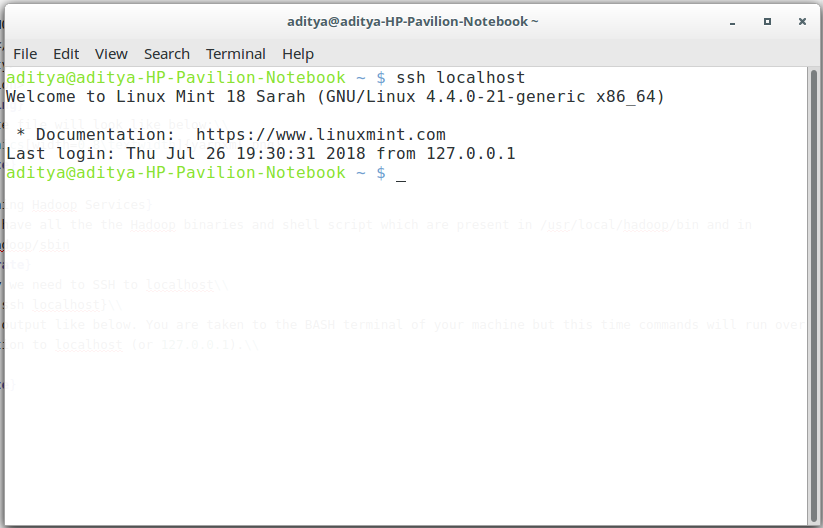
\includegraphics[width=0.8\textwidth]{shssh.png}

\item Before running our cluster for the first time we need to format our namenode\\
\lstinline{$ hadoop namenode -format}\\
You will receive the below output:\\
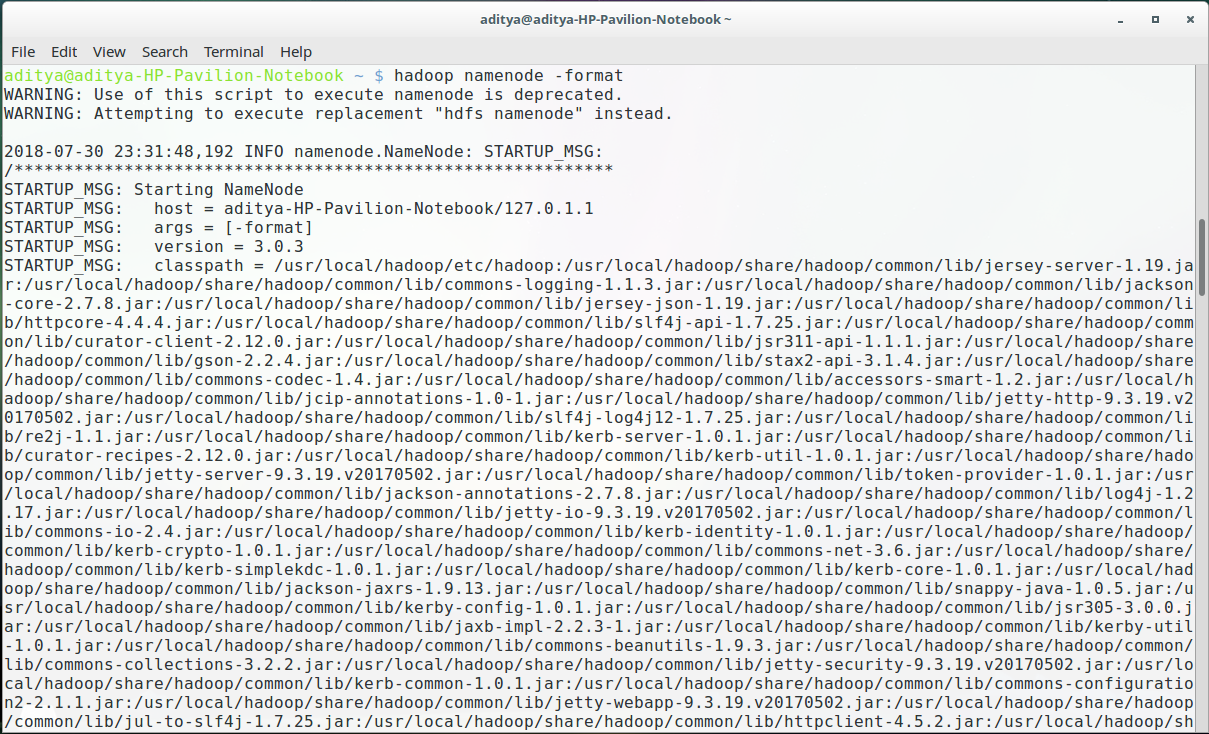
\includegraphics[width=0.8\textwidth]{namenodeformat.png}

\item Now to start the HDFS file system with  its Namenodes and Datanodes enter the following command.\\
\lstinline{$ start-dfs.sh}\\
You will receive the below output:\\
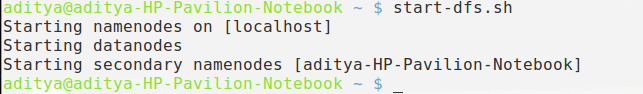
\includegraphics[width=0.8\textwidth]{startdfs.png}


\item Now to start the Yarn resource manager type.\\
\lstinline{$ start-yarn.sh}\\
You will receive the below output:\\
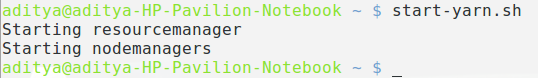
\includegraphics[width=0.8\textwidth]{startyarn.png}


\item Using \emph{jps} command we can see all the running services\\
\lstinline{$ jps}\\
You will receive the below output:\\
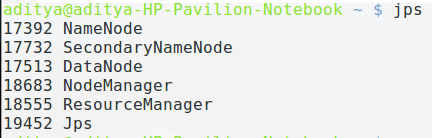
\includegraphics[width=0.8\textwidth]{jpsout.png}

\item Open \emph{http://localhost:9870} in browser to see the Namenode interface.\\
You will receive the below output:\\
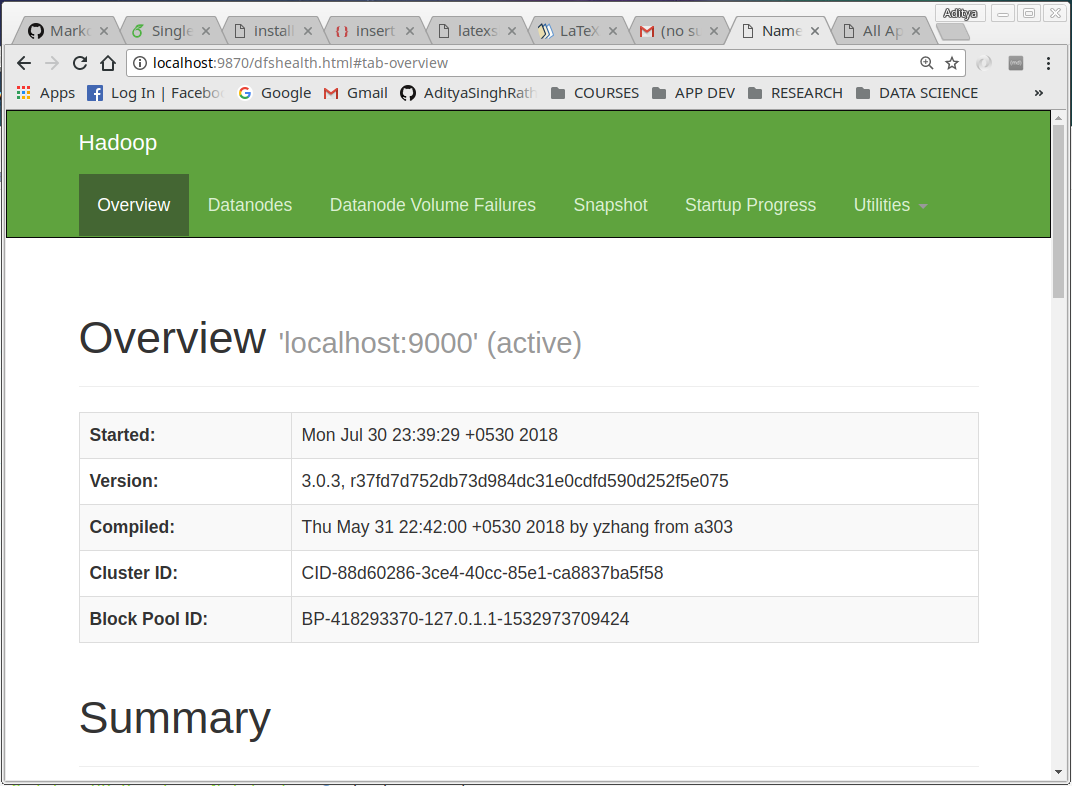
\includegraphics[width=0.8\textwidth]{hadooprun.png}


\item Open \emph{http://localhost:8088} in browser to see the Cluster interface.\\
You will receive the below output:\\
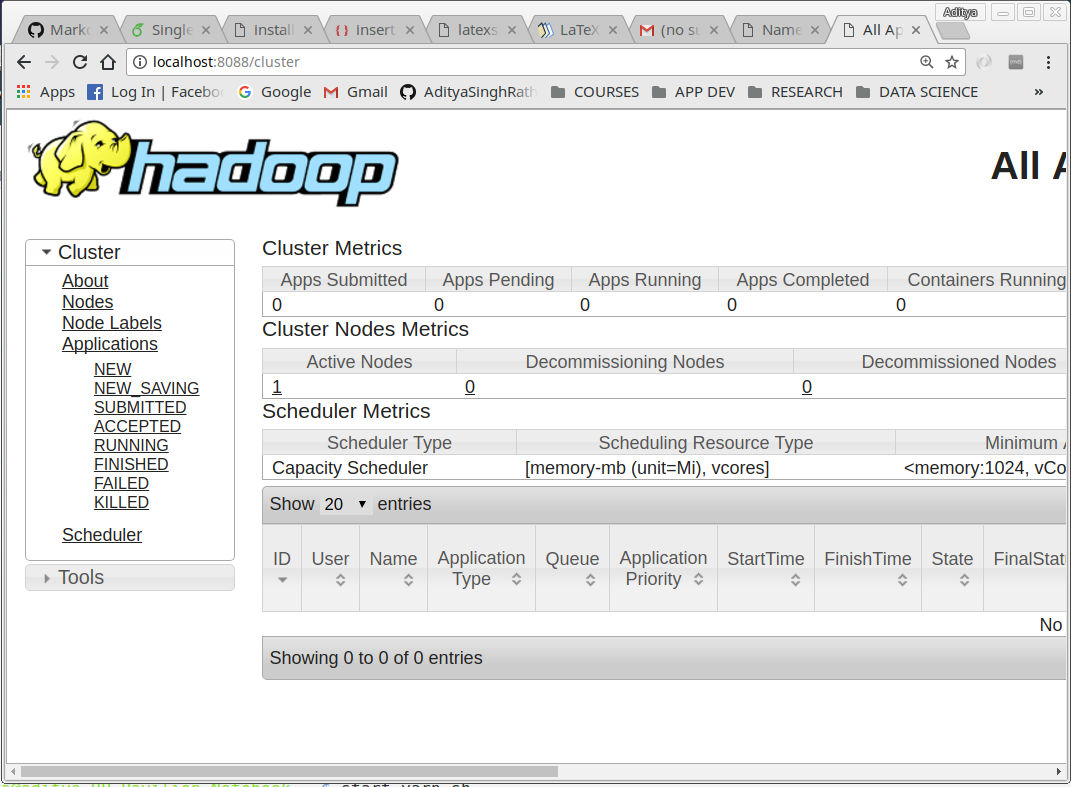
\includegraphics[width=0.8\textwidth]{clusterrun.png}

\end{enumerate}

\section{Conclusion and Stopping}
\textbf{Congratulations !}, Your Linux Mint 18 Machine has a fully functional single Node Hadoop 3.0.3 cluster up and running.\\
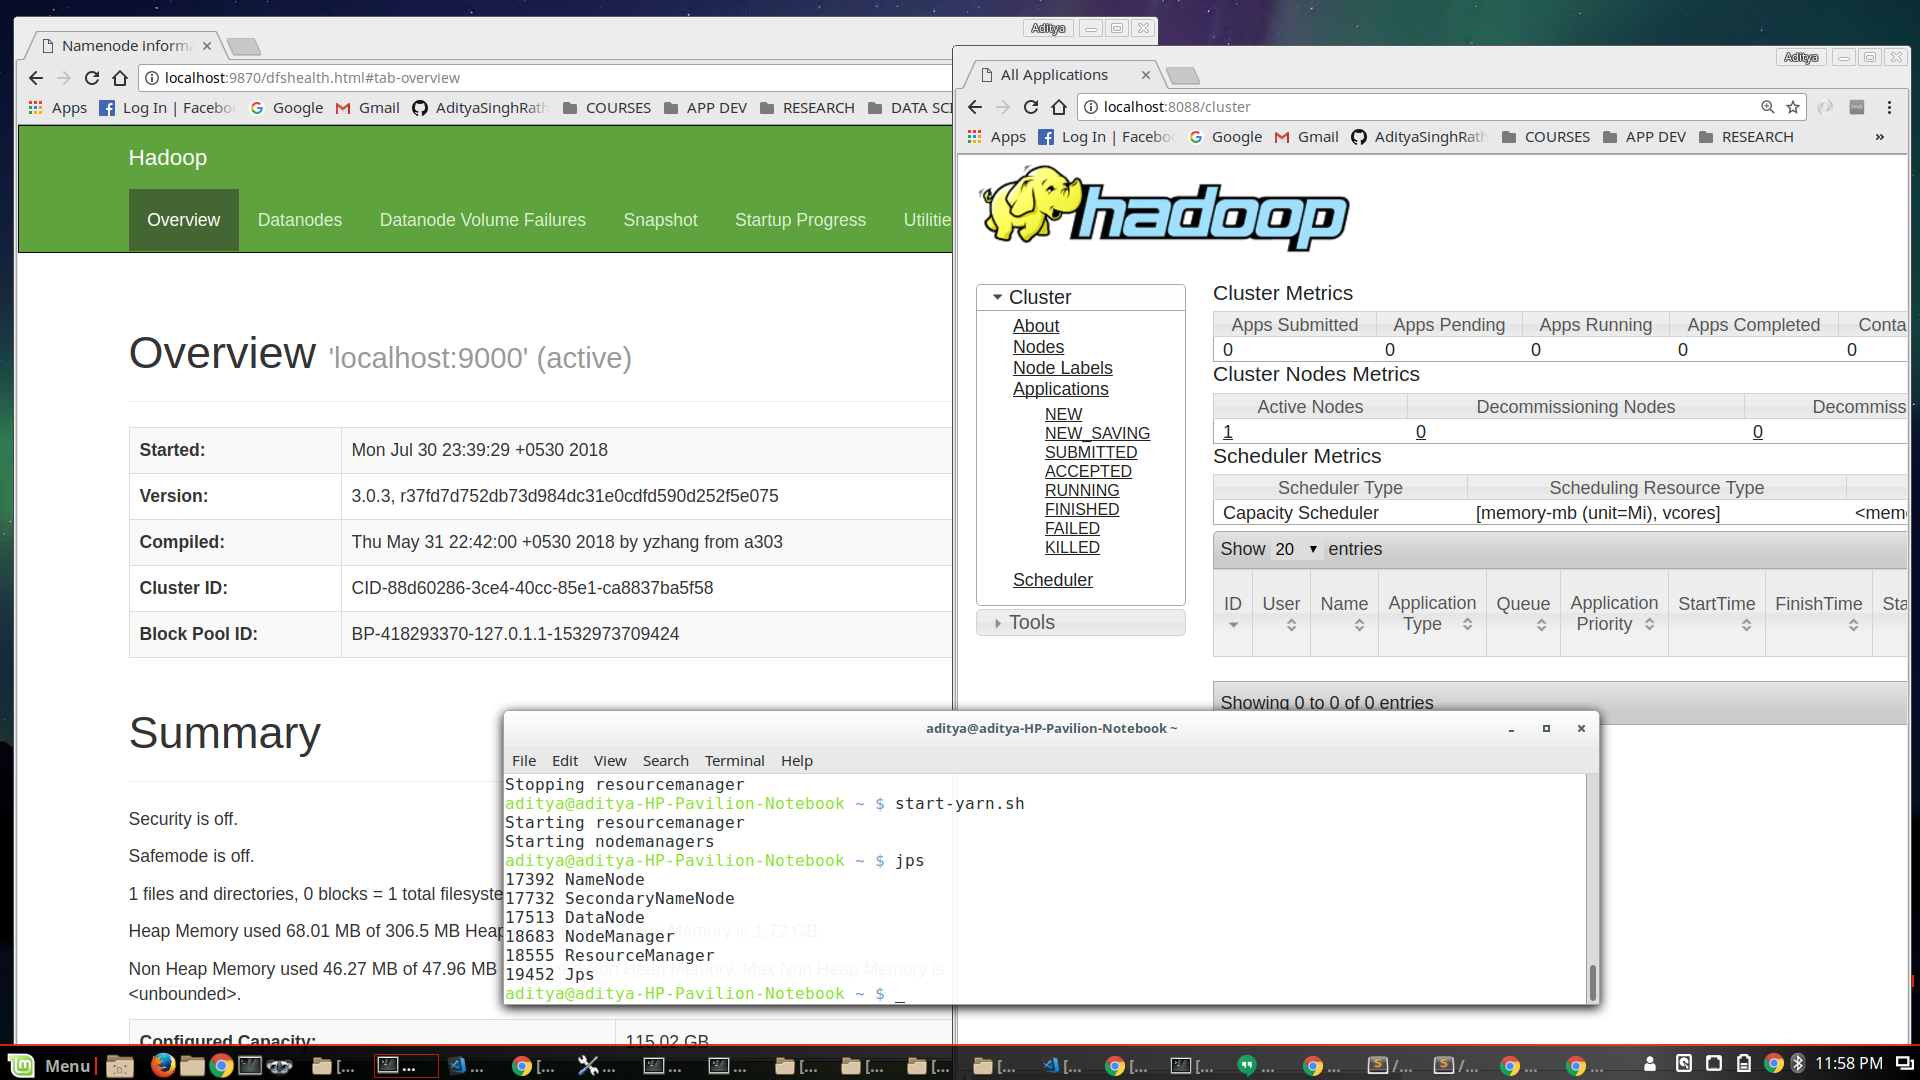
\includegraphics[width=\textwidth]{conclu.png}
\\ Next up we will run a simple MapReduce Wordcount example on our Cluster. For now use the following commands to stop the cluster.                    
                       
\begin{enumerate}
\item To start the HDFS file system enter the following command.\\
\lstinline{$ stop-dfs.sh}\\
You will receive the below output:\\
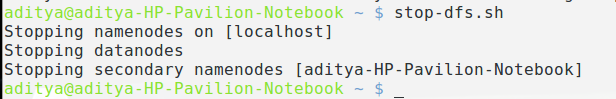
\includegraphics[width=0.8\textwidth]{stopdfs.png}


\item To stop the Yarn resource manager type.\\
\lstinline{$ stop-yarn.sh}\\
You will receive the below output:\\
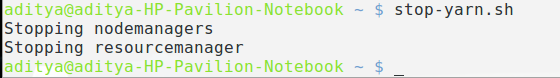
\includegraphics[width=0.8\textwidth]{stopyarn.png}

\end{enumerate}  
  
  
  
  
  
  
  
  
  




\end{document}